\chapter{Dorongan dan Tarikan: Gaya}\label{ch:g2:pushes-and-pulls}

Membuka pintu, menarik ritsleting, menendang bola, dan menyeret
kereta luncur: sepanjang harimu kamu mendorong dan menarik. Fisika
mengumpulkan semuanya di bawah satu nama yang megah --- \omterm{def:g2:pushes-and-pulls:force}{gaya} --- lalu
mengajukan dua pertanyaan sederhana: apa yang dapat dilakukan sebuah
\omterm{def:g2:pushes-and-pulls:force}{gaya}, dan ke arah mana ia bekerja?

\section{Dorongan dan tarikan di mana-mana}

\begin{definition}[Gaya]\label{def:g2:pushes-and-pulls:force}
Sebuah dorongan atau tarikan disebut \emph{gaya}\index{gaya}.
Mendorong ayunan, menarik gerobak, menekan bel pintu,
meregangkan karet gelang, meremas adonan: setiap satunya adalah gaya yang sedang
bekerja. Sebuah gaya selalu punya kekuatan --- lembut atau perkasa ---
dan sebuah \emph{arah}: ia mendorong atau menarik \emph{ke suatu arah}.
\end{definition}

\begin{example}[Dorongan atau tarikan?]\label{ex:g2:pushes-and-pulls:sort}
Pilahlah harimu: menendang bola --- dorongan dengan kaki. Membuka
laci --- tarikan. Menutupnya --- dorongan. Menarik ritsleting jaket
--- tarikan. Menguleni adonan --- banyak dorongan kecil. Tarik tambang
--- dua regu menarik tali yang sama ke arah berlawanan.
\end{example}

\begin{method}[Menggambar gaya sebagai anak panah]\label{met:g2:pushes-and-pulls:arrow}
Para fisikawan menggambar \omterm{def:g2:pushes-and-pulls:force}{gaya} sebagai sebuah \emph{anak panah}:
\begin{enumerate}
  \item anak panah dimulai di tempat dorongan atau tarikan itu
        mencengkeram bendanya;
  \item ia menunjuk ke arah kerja \omterm{def:g2:pushes-and-pulls:force}{gayanya};
  \item \omterm{def:g2:pushes-and-pulls:force}{gaya} yang lebih kuat mendapat anak panah yang lebih panjang.
\end{enumerate}
Satu anak panah kecil menceritakan seluruh kisahnya: di mana, ke arah
mana, seberapa kuat. Kita akan menggambar anak panah ini
bertahun-tahun lamanya.
\end{method}

\begin{omfigure}
\begin{tikzpicture}[scale=0.85]
  \draw[thick] (0,0) -- (4.6,0);
  \draw[thick, fill=omMeth, fill opacity=0.4] (1.4,0) rectangle (2.9,1.0);
  \draw[-Stealth, very thick, omThm] (0.2,0.5) -- (1.3,0.5);
  \node[below, font=\small] at (2.3,-0.25) {dorongan lembut: anak panah pendek};
  \draw[thick] (6.4,0) -- (11.0,0);
  \draw[thick, fill=omMeth, fill opacity=0.4] (8.4,0) rectangle (9.9,1.0);
  \draw[-Stealth, very thick, omThm] (6.5,0.5) -- (8.3,0.5);
  \node[below, font=\small] at (8.7,-0.25) {dorongan perkasa: anak panah panjang};
\end{tikzpicture}

{\small Kotak yang sama didorong dua kali. Anak panah menunjukkan di
mana dorongan mencengkeram, ke arah mana ia bekerja, dan --- lewat
panjangnya --- seberapa kuat.}
\end{omfigure}

\begin{omfigure}
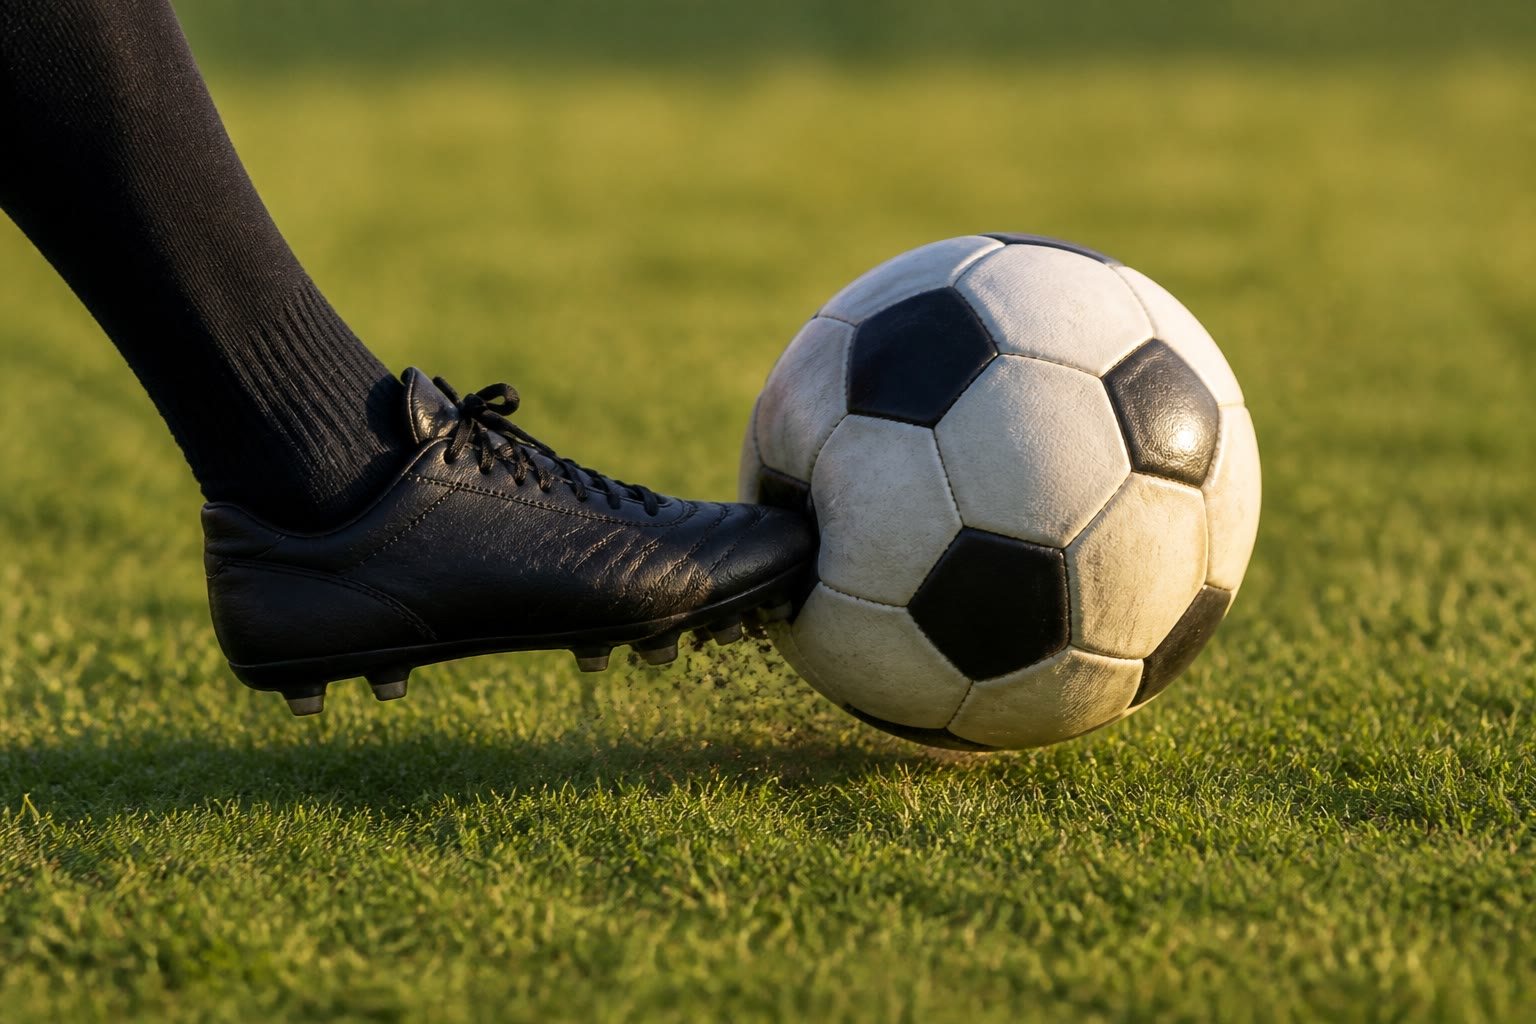
\includegraphics[width=0.58\linewidth]{images/book1/ai/g2-pushes-kick.jpg}

{\small Sebuah \omterm{def:g2:pushes-and-pulls:force}{gaya} pada saat ia bekerja: sepatu bot mendorong, dan bola yang tadinya diam sebentar lagi melesat.}
\end{omfigure}

\section{Apa yang dilakukan gaya}

\begin{proposition}[Empat pekerjaan sebuah gaya]\label{prop:g2:pushes-and-pulls:jobs}
Sebuah \omterm{def:g2:pushes-and-pulls:force}{gaya} dapat melakukan empat hal pada sebuah benda:
\begin{enumerate}
  \item \emph{menggerakkannya} --- tendangan mengirim bola yang
        tadinya diam melesat pergi;
  \item \emph{menghentikannya} --- tangan penjaga gawang menghentikan
        tembakan;
  \item \emph{membelokkannya} --- ketukan dari samping membengkokkan
        lintasan bola yang menggelinding;
  \item \emph{mengubah bentuknya} --- remasan memipihkan spons,
        tarikan meregangkan karet gelang.
\end{enumerate}
Tanpa \omterm{def:g2:pushes-and-pulls:force}{gaya}, tidak ada satu pun dari keempatnya: benda yang dibiarkan
sendirian sama sekali akan tetap melakukan persis apa yang tadi
dilakukannya.
\end{proposition}

\begin{omfigure}
\begin{tikzpicture}[scale=0.85]
  \draw[dashed, omExo] (0,0.6) -- (4.2,0.6);
  \fill[omDef] (0.6,0.6) circle (0.24);
  \fill[omDef, opacity=0.45] (3.0,0.6) circle (0.24);
  \draw[-Stealth, very thick, omThm] (4.2,0.6) -- (6.0,1.7);
  \fill[omDef, opacity=0.45] (5.4,1.33) circle (0.24);
  \draw[-Stealth, thick, omThm] (4.2,-0.35) -- (4.2,0.5);
  \node[below, font=\small, omThm] at (4.2,-0.5) {ketukan dari samping di sini};
  \node[below, font=\small] at (1.4,0.3) {menggelinding lurus};
  \node[right, font=\small] at (5.85,2.05) {arah baru!};
\end{tikzpicture}

{\small Pekerjaan nomor tiga: bola yang menggelinding mendapat ketukan
dari samping dan lintasannya membengkok ke arah dorongan itu.}
\end{omfigure}

\begin{example}[Gaya lebih kuat, akibat lebih besar]\label{ex:g2:pushes-and-pulls:stronger}
Ketuklah sebutir kelereng: ia bergulir sampai ke tepi meja. Sentillah
kuat-kuat: ia melesat melintasi ruangan. Kelereng yang sama, jari yang
sama --- hanya kekuatan dorongannya yang berubah, dan penerbangan
kelereng itu berubah bersamanya. \omterm{def:g2:pushes-and-pulls:force}{Gaya} lembut, akibat lembut; \omterm{def:g2:pushes-and-pulls:force}{gaya}
perkasa, akibat perkasa.
\end{example}

\begin{example}[Cobalah: para pengubah bentuk]\label{ex:g2:pushes-and-pulls:shape}
Kumpulkan spons, karet gelang, segumpal plastisin, dan balok kayu.
Remas dan regangkan masing-masing. Spons melenting kembali begitu kamu
lepaskan; karet gelang pun begitu. Plastisin mempertahankan bentuk
barunya --- gayamu membuat lekukan selamanya. Dan baloknya? Remasan
terkuatmu sama sekali tidak mengubahnya (setidaknya yang dapat kamu
lihat!). Setiap benda menjawab \omterm{def:g2:pushes-and-pulls:force}{gaya} dengan caranya sendiri.
\end{example}

\section{Gaya tanpa sentuhan}

\begin{example}[Tarikan Bumi]\label{ex:g2:pushes-and-pulls:earthpull}
Jatuhkan sebuah sendok: ia turun. Lemparkan bola setinggi yang kamu
mau: ia kembali turun. Daun, tetes hujan, remah roti --- semua yang
dilepaskan jatuh \emph{ke bawah}. Ada sesuatu yang menarik semuanya,
sepanjang waktu, tanpa menyentuhnya: Bumi itu sendiri. Tarikan Bumi
adalah \omterm{def:g2:pushes-and-pulls:force}{gaya} yang paling ajek dalam hidupmu --- ia tidak pernah
melepaskan, dan itulah sebabnya ``bawah'' berarti hal yang sama di
seluruh halaman bermain.
\end{example}

\begin{omfigure}
\begin{tikzpicture}[scale=0.85]
  % the falling apple
  \draw[thick] (0,0) -- (5.0,0);
  \draw[thick, red!60!black, fill=red!70] (1.4,2.5) circle (0.32);
  \draw[thick, brown!60!black]
    (1.4,2.82) .. controls (1.45,2.98) .. (1.56,3.08);
  \draw[thick, green!45!black, fill=green!45]
    (1.62,3.02) ellipse [x radius=0.16, y radius=0.07, rotate=30];
  \draw[-Stealth, very thick, omDef] (1.4,2.05) -- (1.4,1.1);
  \node[right, font=\small, omDef] at (1.65,1.6)
    {Bumi menarik ke bawah};
  \node[below, font=\small] at (2.5,-0.25)
    {apel jatuh: ditarik, bukan didorong};
  % the magnet holding a paperclip up across a gap
  \draw[thick, fill=red!70] (7.9,2.35) rectangle (8.75,2.95);
  \draw[thick, fill=blue!60] (8.75,2.35) rectangle (9.6,2.95);
  \begin{scope}[shift={(8.54,1.65)}, rotate=-90]
    \draw[thick, rounded corners=2.6pt]
      (0,0) -- (1.1,0) -- (1.1,0.42) -- (0.12,0.42) -- (0.12,0.14)
      -- (0.95,0.14) -- (0.95,0.30) -- (0.30,0.30);
  \end{scope}
  \draw[-Stealth, very thick, omDef] (9.15,1.0) -- (9.15,2.0);
  \node[below, font=\small] at (8.75,0.1)
    {magnet menarik ke atas --- tanpa sentuhan};
\end{tikzpicture}

{\small Dua \omterm{def:g2:pushes-and-pulls:force}{gaya} tanpa sentuhan: Bumi menarik apel ke bawah menembus
\omterm{def:g2:air-around-us:air}{udara}; \omterm{def:g1:magnets:magnet}{magnet} menarik penjepit ke atas menembus \omterm{def:g2:air-around-us:air}{udara}.}
\end{omfigure}

\begin{remark}[Kawan lama]\label{rem:g2:pushes-and-pulls:magnets}
Kamu sudah mengenal satu lagi \omterm{def:g2:pushes-and-pulls:force}{gaya} tanpa sentuhan: \omterm{def:g1:magnets:magnet}{magnet}, yang
menarik penjepit kertasnya melintasi celah \omterm{def:g2:air-around-us:air}{udara}. \omterm{def:g1:magnets:magnet}{Magnet} dan tarikan
Bumi adalah dua \omterm{def:g2:pushes-and-pulls:force}{gaya} tanpa sentuhan dalam kehidupan sehari-harimu ---
kekecualian yang langka dan berharga, sebab setiap dorongan atau
tarikan lain yang kamu temui memerlukan sentuhan. Keduanya akan tumbuh
menjadi bab yang besar di bagian akhir pelajaran ini.
\end{remark}

\section{Latihan}

\begin{exercise}[$\star$]\label{exo:g2:pushes-and-pulls:1}
Dorongan atau tarikan? Membunyikan bel pintu; \ membuka laci;
\ menyundul bola; \ menyeret kereta luncur mendaki; \ memencet pasta
gigi.
\end{exercise}

\begin{exercise}[$\star$]\label{exo:g2:pushes-and-pulls:2}
Tiga hal apa yang diceritakan sebuah anak panah \omterm{def:g2:pushes-and-pulls:force}{gaya} tentang \omterm{def:g2:pushes-and-pulls:force}{gayanya}?
\end{exercise}

\begin{exercise}[$\star$]\label{exo:g2:pushes-and-pulls:3}
Sebutkan empat pekerjaan sebuah \omterm{def:g2:pushes-and-pulls:force}{gaya}, dan berikan contohmu sendiri
untuk masing-masing --- berbeda dari contoh dalam bab ini.
\end{exercise}

\begin{exercise}[$\star$]\label{exo:g2:pushes-and-pulls:4}
Sebutir kelereng menggelinding lurus ke arahmu. Hanya dengan satu
jari, bagaimana kamu membuatnya: berhenti? \ melaju lebih cepat?
\ membelok ke samping? Katakan ke arah mana jarimu mendorong tiap kali.
\end{exercise}

\begin{exercise}[$\star$]\label{exo:g2:pushes-and-pulls:5}
Mana yang melenting kembali dan mana yang mempertahankan lekukannya:
spons; \ plastisin; \ karet gelang; \ salju yang lembut?
\end{exercise}

\begin{exercise}[$\star$]\label{exo:g2:pushes-and-pulls:6}
Gambarlah sebuah kotak yang didorong lembut ke kanan dan kotak yang
sama didorong kuat ke kiri. Apa bedanya kedua anak panahmu?
\end{exercise}

\begin{exercise}[$\star$]\label{exo:g2:pushes-and-pulls:7}
\omterm{def:g2:pushes-and-pulls:force}{Gaya} apa yang membuat setiap benda yang dijatuhkan turun? Perlukah ia
menyentuh sendok yang jatuh itu? Ke arah mana ia selalu menarik?
\end{exercise}

\begin{exercise}[$\star$]\label{exo:g2:pushes-and-pulls:8}
Sebutkan dua \omterm{def:g2:pushes-and-pulls:force}{gaya} tanpa sentuhan yang sudah kamu temui, masing-masing
dengan satu contoh yang terlihat di rumah.
\end{exercise}

\begin{exercise}[$\star\star$]\label{exo:g2:pushes-and-pulls:9}
Dalam tarik tambang, kedua regu menarik sekuat tenaga, namun pita di
tengah tali kadang sama sekali tidak bergerak. Gambarlah talinya
dengan anak panah kedua regu. Apa yang pasti benar tentang kedua
tarikan itu ketika pitanya diam? Apa yang terjadi begitu satu regu
menarik lebih kuat?
\end{exercise}

\begin{exercise}[$\star\star$]\label{exo:g2:pushes-and-pulls:10}
Bola yang dilempar lurus ke atas melambat, berhenti sekejap mata, lalu
jatuh kembali. \omterm{def:g2:pushes-and-pulls:force}{Gaya} mana yang bekerja ketika naik, di puncak, dan
ketika turun? Apakah \omterm{def:g2:pushes-and-pulls:force}{gaya} itu pernah berhenti menarik? (Gambarlah anak
panahnya pada masing-masing dari ketiga saat itu.)
\end{exercise}
